%!TEX root = ../main.tex
\section{Random walks and preferential attachment}\label{section:random-walk}

\subsection{Theoretical degree distribution}
One of the weaknesses of the BA model and its generalizations is that this implicitly requires a knowledge of the total degree and a calculation across existing vertices on the graph. This requirements then destroys the potential for this model to exhibit emergent properties based on local behaviour. In real-world networks, such as social networks or webpages, the new 'vertices' that join rarely have a global knowledge of the other network vertices. The attachment by performing a random walk is a solution proposed by \citet{Saramaki2004}. In this model, a vertex is chosen at random from existing vertices and then executes a random walk of length $L$ from that vertex. The new vertex then attaches to the destination vertex. 

Preferential attachment then follows from the fact that the random walker is more likely to end up at a more highly connected vertex. This models real-world models such as interconnected webpages better, since we are likely to click on links to webpages from webpages we are already visiting. 

This model was thought to be able to reproduce the BA degree distribution even for $L=1$ \citep{Saramaki2004,J.P.Saramaki2004}. While this is the case for large $L$, \citet{Cannings2013} later showed that the $L=1$ and $m=1$ degree sequence converges to a degenerate limiting solution in which almost every vertex has degree 1, instead of a power law distribution, and demonstrated that this model is fundamentally different from the BA model, unless we allow an indefinite length for the random walk. For $L = 0$, this reduces to the random attachment model. 

\subsection{Numerical simulation}

A few considerations were taken into account when writing the numerical simulation for the random walk:

\begin{enumerate}
	\item We are adding $m$ edges to each new vertex. Should we reset the random walk to find each new destination vertex, or should we continue an $L$-step random walk from the current destination vertex to the next destination vertex till we get $m$ edges?
	\item Is the walker allowed to trace his steps backwards, that is, is the walk self-avoiding?
\end{enumerate}

For point 1, we followed the convention in \citet{Saramaki2004} where we continue the random walk from the previous destination vertex, until we reach $m$ destination vertices, that is, the random walk only resets when a new vertex is added. For point 2, it was decided that the walk will not be self-avoiding, otherwise it would get stuck easily. 

For $L=0$, the degree distribution reduces to that of random attachment, as expected. 

The raw degree distribution generated by $L = 1$ is shown in \autoref{fig:rw-fixed-n-degree-dist}, with the dotted lines showing the theoretical BA distribution for the same $m$. We can see quite clearly that the case of $m = 1$ does not follow a power law distribution of preferential attachment. 

\begin{figure}
    \centering
    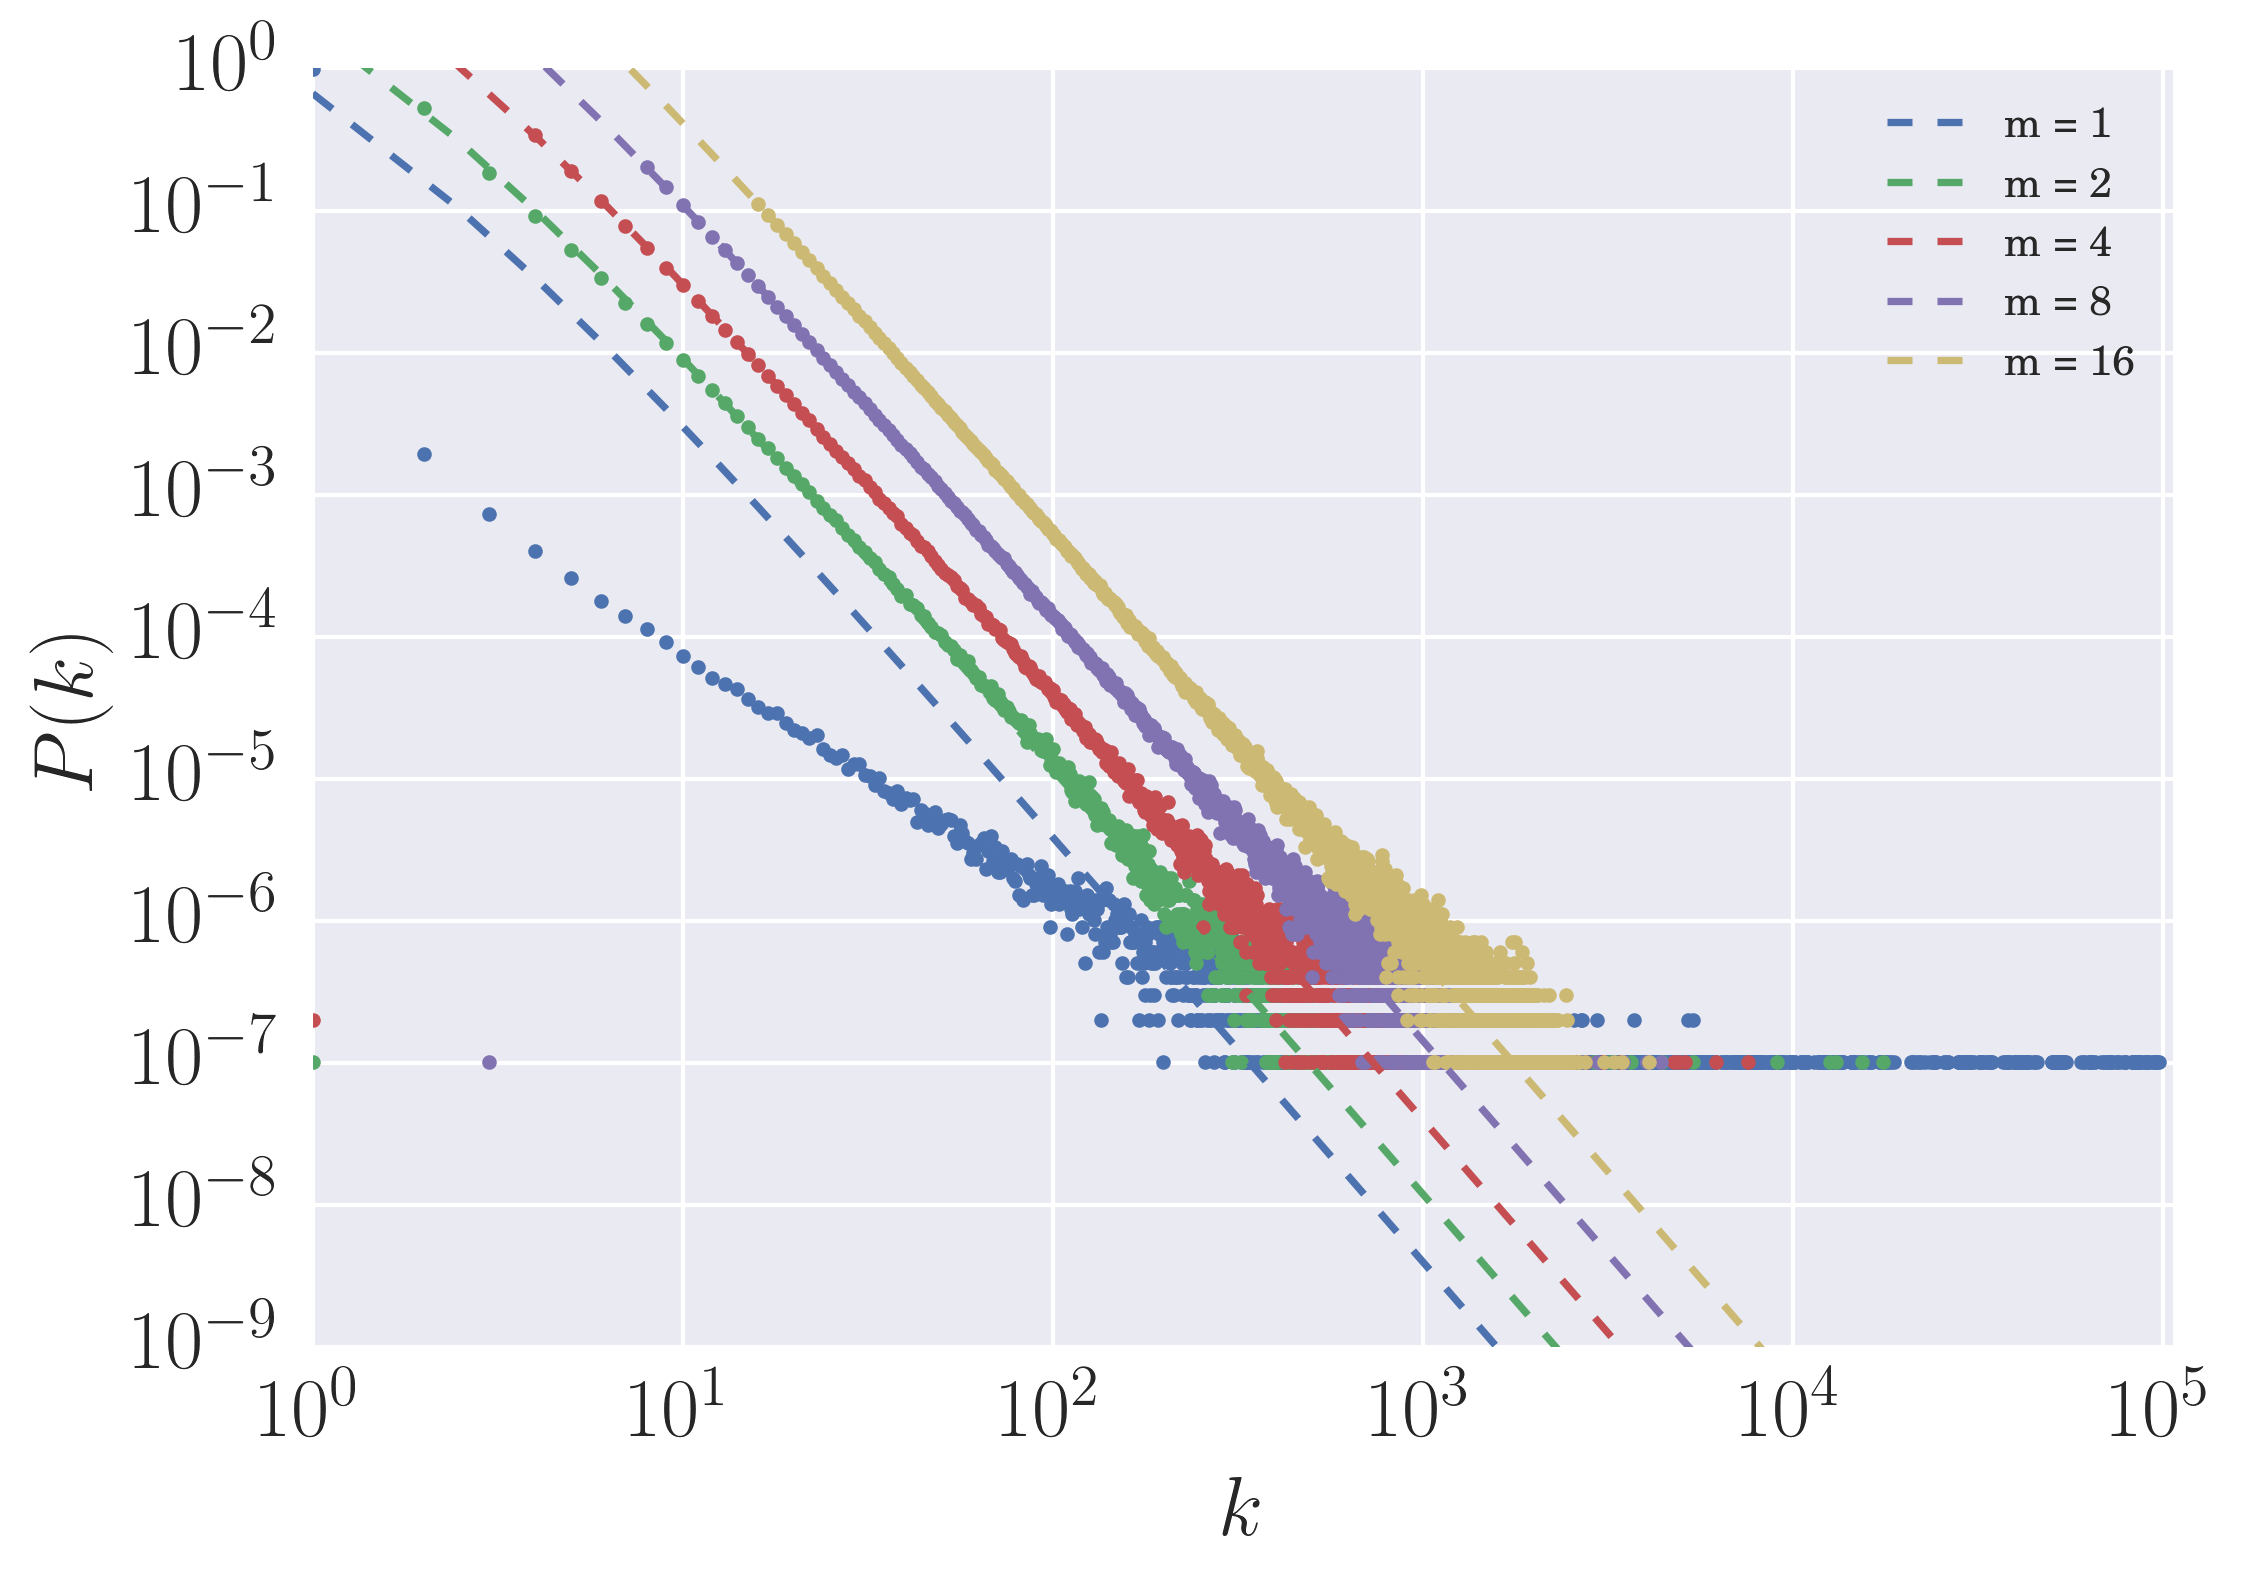
\includegraphics[height=0.5\linewidth]{img/rw-fixed-n-degree-dist}
    \caption{Degree distribution of the random walk model for $N=10^5$, $L=1$, and varying $m$}
    \label{fig:rw-fixed-n-degree-dist}
\end{figure}

To test whether it follows a power law distribution, we can use the same technique in \autoref{subsection:ppa-numerical-analysis}, that is, compare its KS-statistic against those of synthetic data, measured against a reference theoretical distribution. This was first done for $L=1$, $N=10^5$, and various values of $m$, and the following p-values were obtained:

\begin{center}
\begin{tabular}{ c | c}
m & $p$-value \\
\hline
1 & 0.00 \\
2 & 0.00 \\
4 & 0.029 \\
8 & 0.768 \\
16 & 0.648 \\
\end{tabular}
\label{table:rw-kstest}
\end{center} 

As we can see from the table, for small $m$. Indeed, this was verified by \citet{Cannings2013} who showed that in this case, the degree distribution converges to a degenerate limiting solution in which almost every vertex has degree 1. At $m=8$, however, it is already highly plausible that the degree distribution follows that of the preferential attachment model. 

Numerical simulations were done for fixed $N$ and fixed $m$ but varying $L$ from 1 to 8, with the $m$ chosen to be $8$ from the previous results and $N = 10^5$. The same technique was used to test whether it follows a power law distribution, and we obtain the result of $p = 0.64$ for all $L$. This shows that it is plausible that the degree distribution for the random walk attachment follows a power law, and this holds regardless of $L$. 